\documentclass[b1]{sciposter}
\usepackage{epsfig} 
\usepackage[english]{layout}
\usepackage[english]{babel}
\usepackage{multicol}
\usepackage[utf8]{inputenc}
\usepackage{ae,aecompl}
\usepackage{amsmath,amssymb,latexsym, cancel}
\usepackage{amssymb,latexsym}
\usepackage{graphicx}
\usepackage{float}
\usepackage{blindtext}
\usepackage{array}
\usepackage[small,sf]{caption}
%\usepackage{fancybullets}
\newtheorem{Def}{Definition}
\definecolor{BoxCol}{rgb}{0.9,0.9,0.9} % uncomment for grey background to \section boxes % for use with default option boxedsections
%\definecolor{BoxCol}{rgb}{0.9,0.9,1} % uncomment for light blue background to \section boxes % for use with default option boxedsections
%\definecolor{SectionCol}{rgb}{0,0,0.5} % uncomment for dark blue \section text
%\renewcommand{\titlesize}{\LARGE} %\renewcommand{\authorsize}{\Large} %\renewcommand{\instsize}{\large}
\title{\Huge{Título del Poster}}
% Note: only give author names, not institute
\author{José Mejía $^{1,\dagger}$, Secon Author$^{2}$, and Third Author$^{3}$}
 % insert correct institute name
\institute{$^{1}$Departamento de F\'{\i}sica, Univ. de Los  Andes, 111711 Bogot\'a, Colombia. \\ $^{2}$Departamento de F\'{\i}sica
Te\'orica II. Univ. Complutense. 28040 Madrid. Spain. \\ $^{3}$Departamento de F\'{\i}sica, Univ. Nacional de Colombia, 111321 Bogot\'a, Colombia.} \email{$^{\dagger}$jr.mejia1228@uniandes.edu.co} % shows author email address below institute %\date is unused by the current \maketitle
% The following commands can be used to alter the default logo settings

\leftlogo[1.5]{header_3_1} % defines logo to left of title (with scale factor) 
%\rightlogo[0.52]{RuGlogo} 
% same but on right
% NOTE: This will require presence of files logoWenI.eps and RuGlogo.eps, % or other supported format in the current directory %%%%%%%%%%%%%%%%%%%%%%%%%%%%%%%%%%%%%%%%%%%%%%%%%%%%%%%%%%%%%%%%%%%%%%%%%%%%%%%% %%% Begin of Document

\rightlogo[1.2]{escudo}

\begin{document} 
%define conference poster is presented at (appears as footer)
\conference{\textit{Laboratorio Intermedio, 2017 Universidad de los Andes}}
\maketitle
\begin{abstract}


\blindtext
 

\end{abstract}
%%% Begin of Multicols-Enviroment
\begin{multicols}{2}

\section{Introduction and Formalism}

\blindtext    


\begin{figure}[H]
\centering
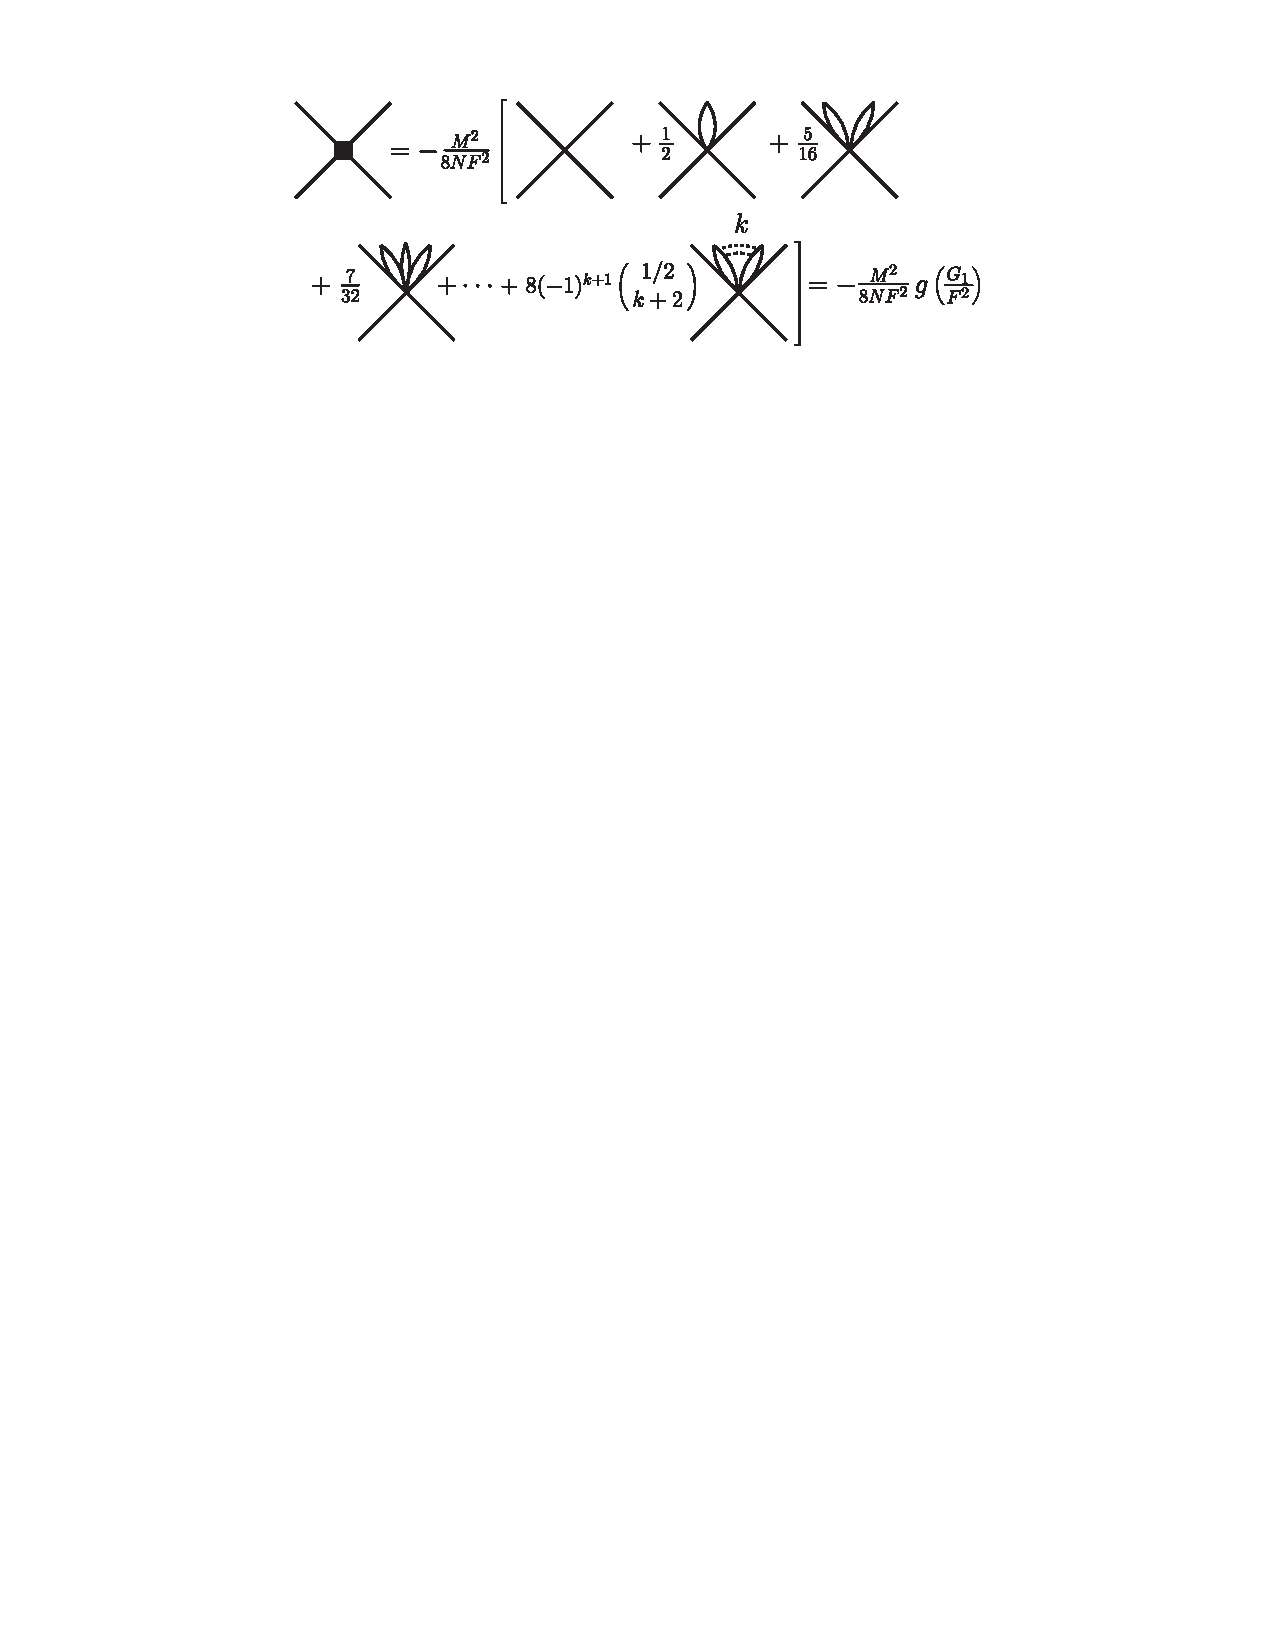
\includegraphics[scale=2.0]{massvertex.pdf}
\label{fig:massvertex}
\end{figure}


This vertex takes into account all possible insertions of thermal tadpoles coming from diagrams with six or more external legs. Its Feynman rule is written in terms of a function $g(x)$ that reads


\begin{equation}
g(x)=-\frac{8}{x^2}\left[\sqrt{1-x}-1+\frac{x}{2}\right]=-8\sum_{k=0}^{\infty}(-1)^k \begin{pmatrix} 1/2\cr k+2 \end{pmatrix} x^k=1+\frac{x}{2}+\frac{5}{16}x^2+\cdots
\label{eqn:massvert}
\end{equation}

$G_{1}(M,T)$ is taken as in \cite{Gerber:1988tt}. Since this is not a scattering approach, we do not consider any combinatory factor linked with the way the pion lines are attached either with external legs or loops. Now, we are able to diagramatically construct the partition function for $N$ massless pions.

%\centerline{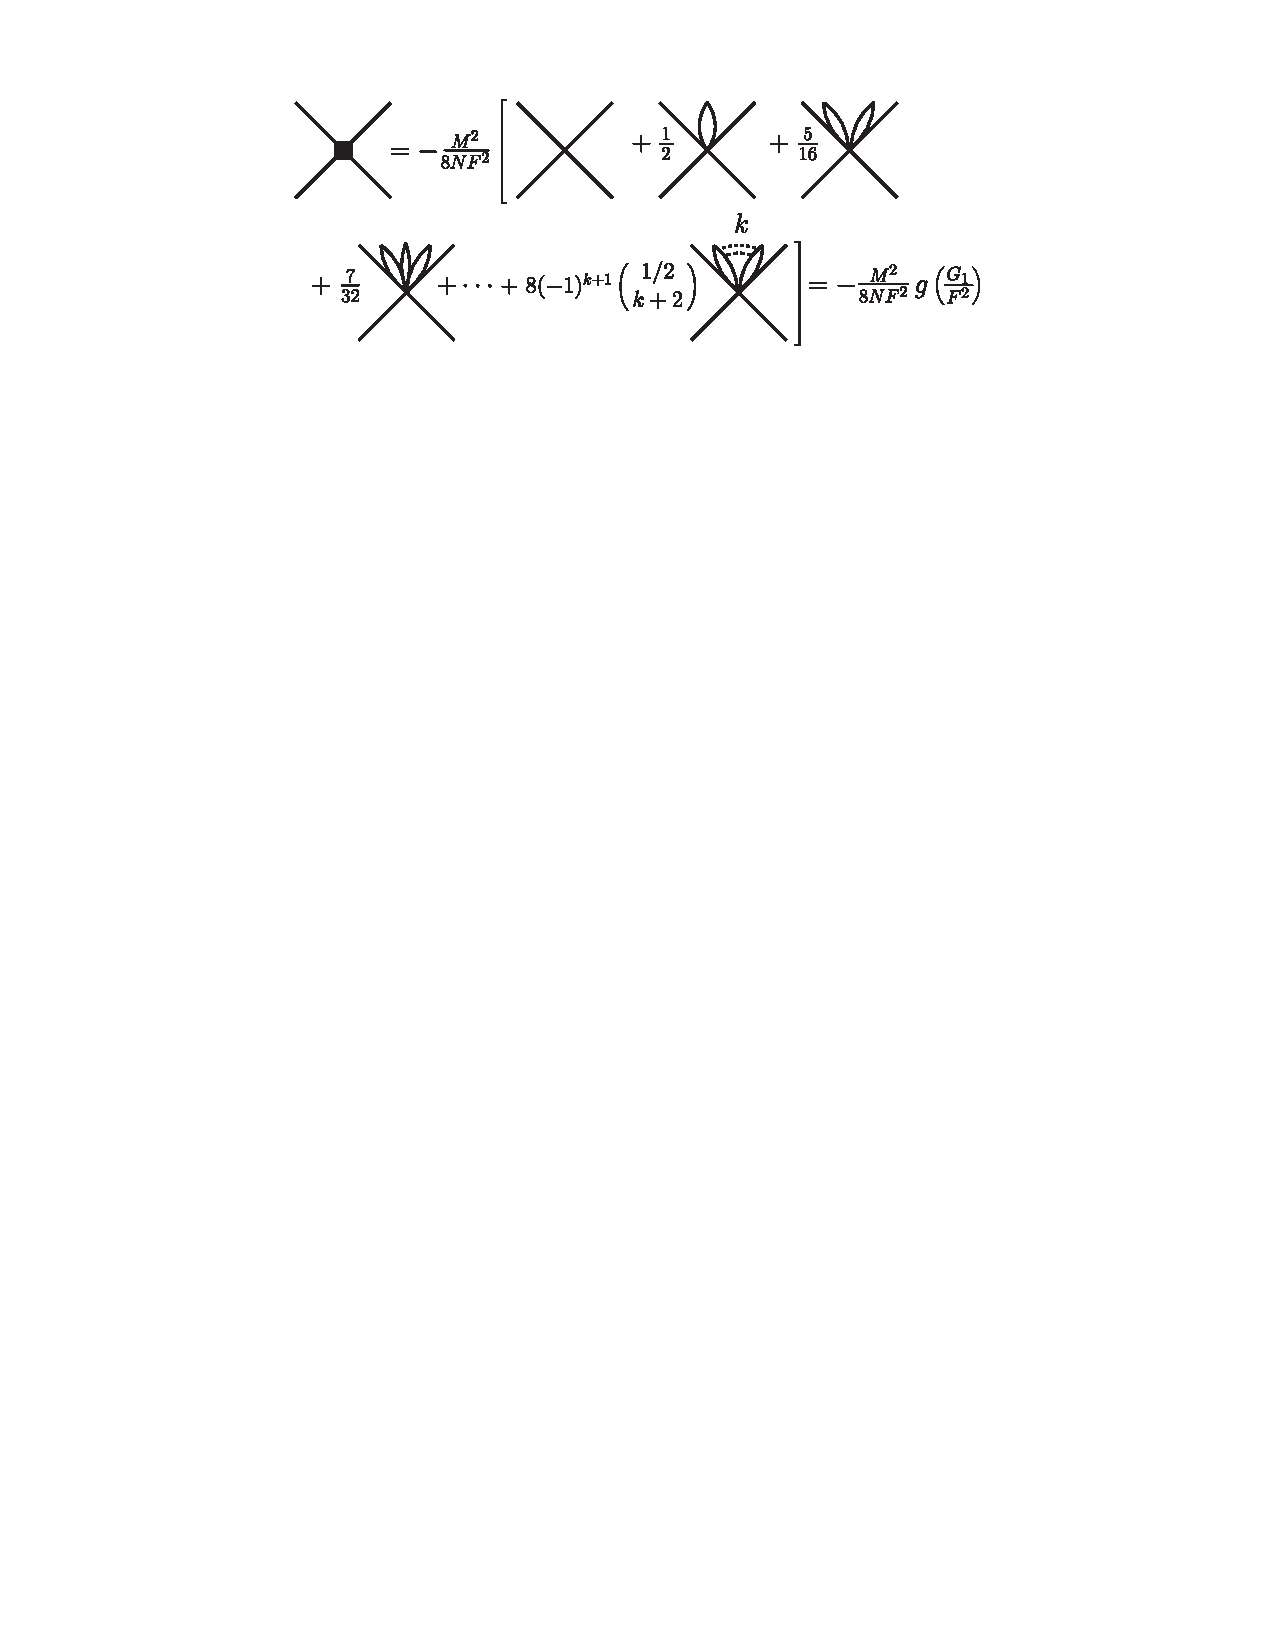
\includegraphics[width=0.4\textwidth]{massvertex.pdf}}

\section{Free Energy and Order Parameters}

\subsection{Free Energy}
\blindtext
\blinddescription


\begin{figure}[]
\centering
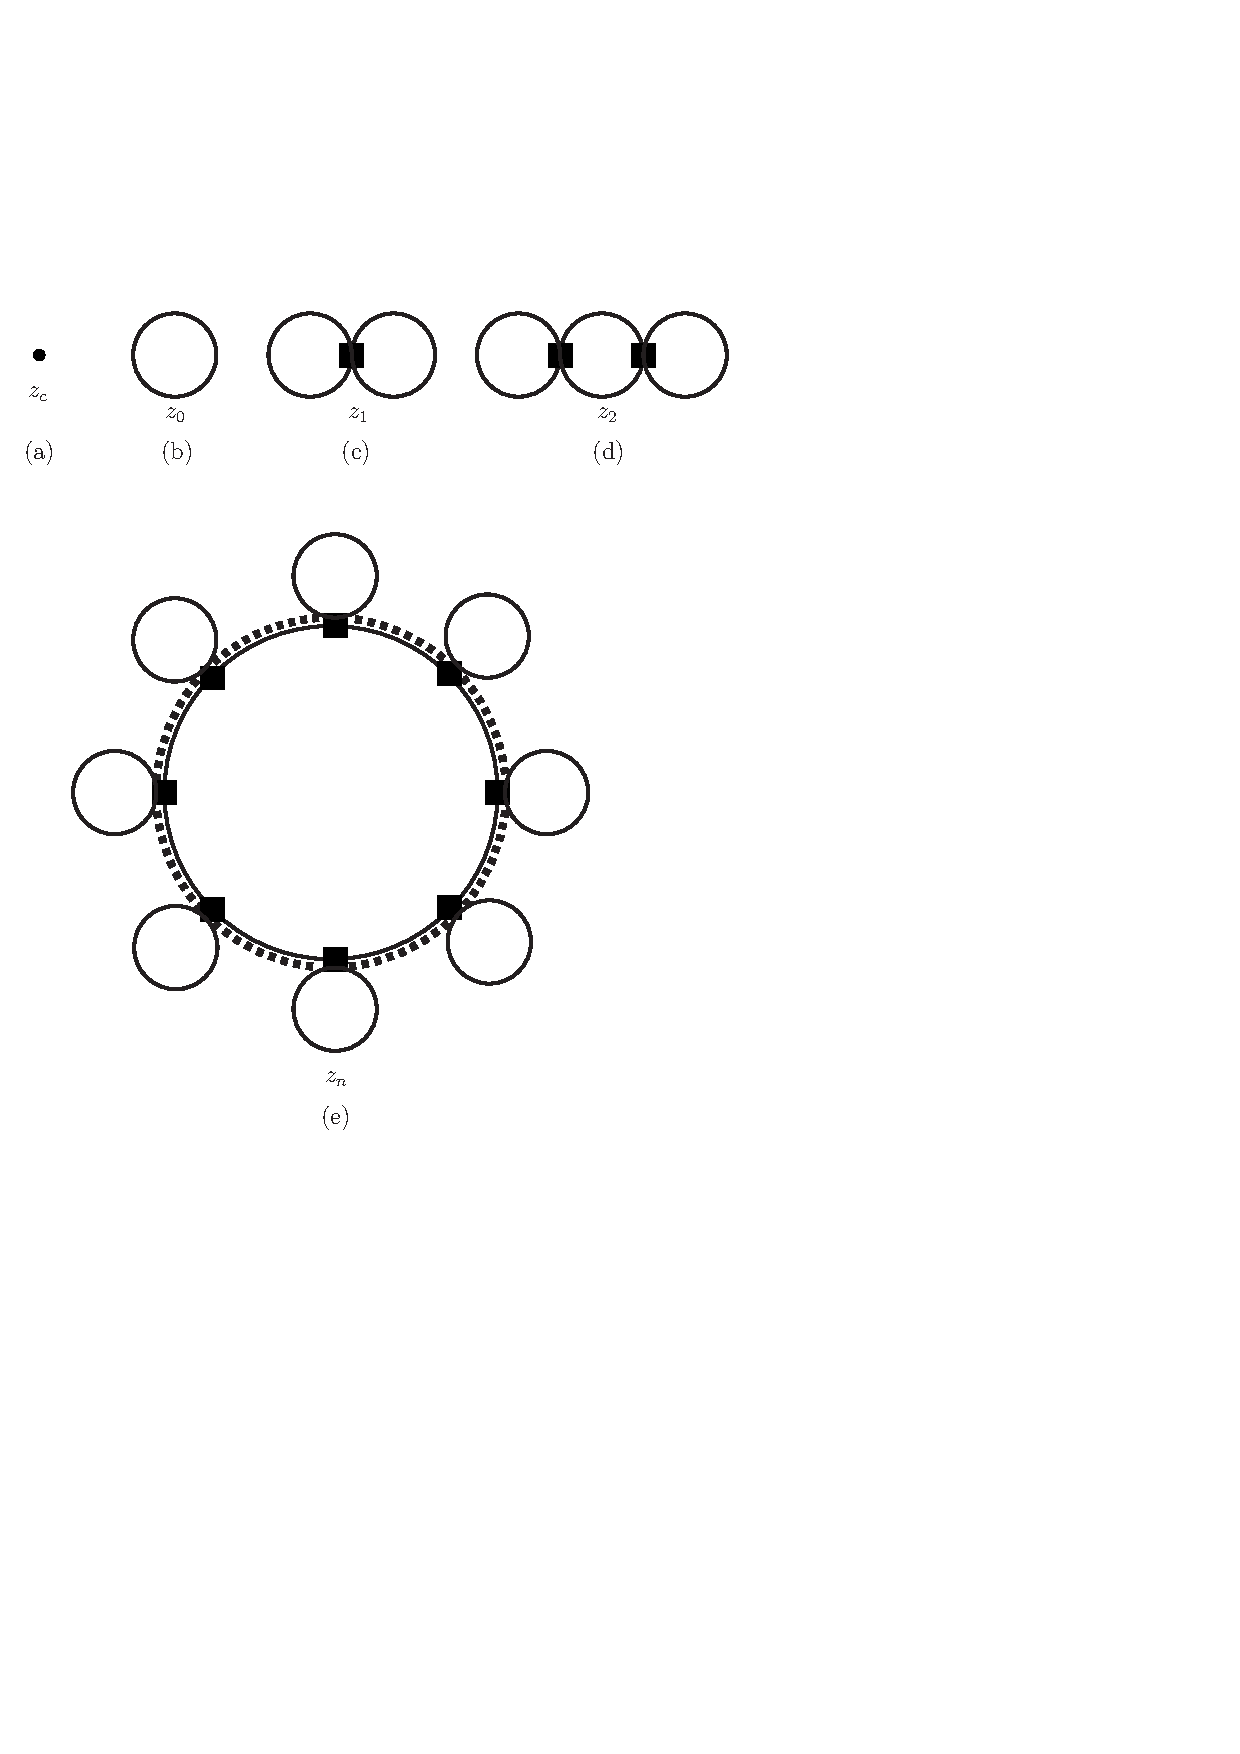
\includegraphics[scale=1.60]{Partition_function.pdf}
\label{fig:partfun}
\end{figure}


\subsection{Scalar Quark Condensate and Susceptibility}

The chiral limit $M\rightarrow 0^{+}$ is plotted in the following figures \cite{Cortes:2016ecy}.

\begin{figure}[H]
\begin{center}
\centerline{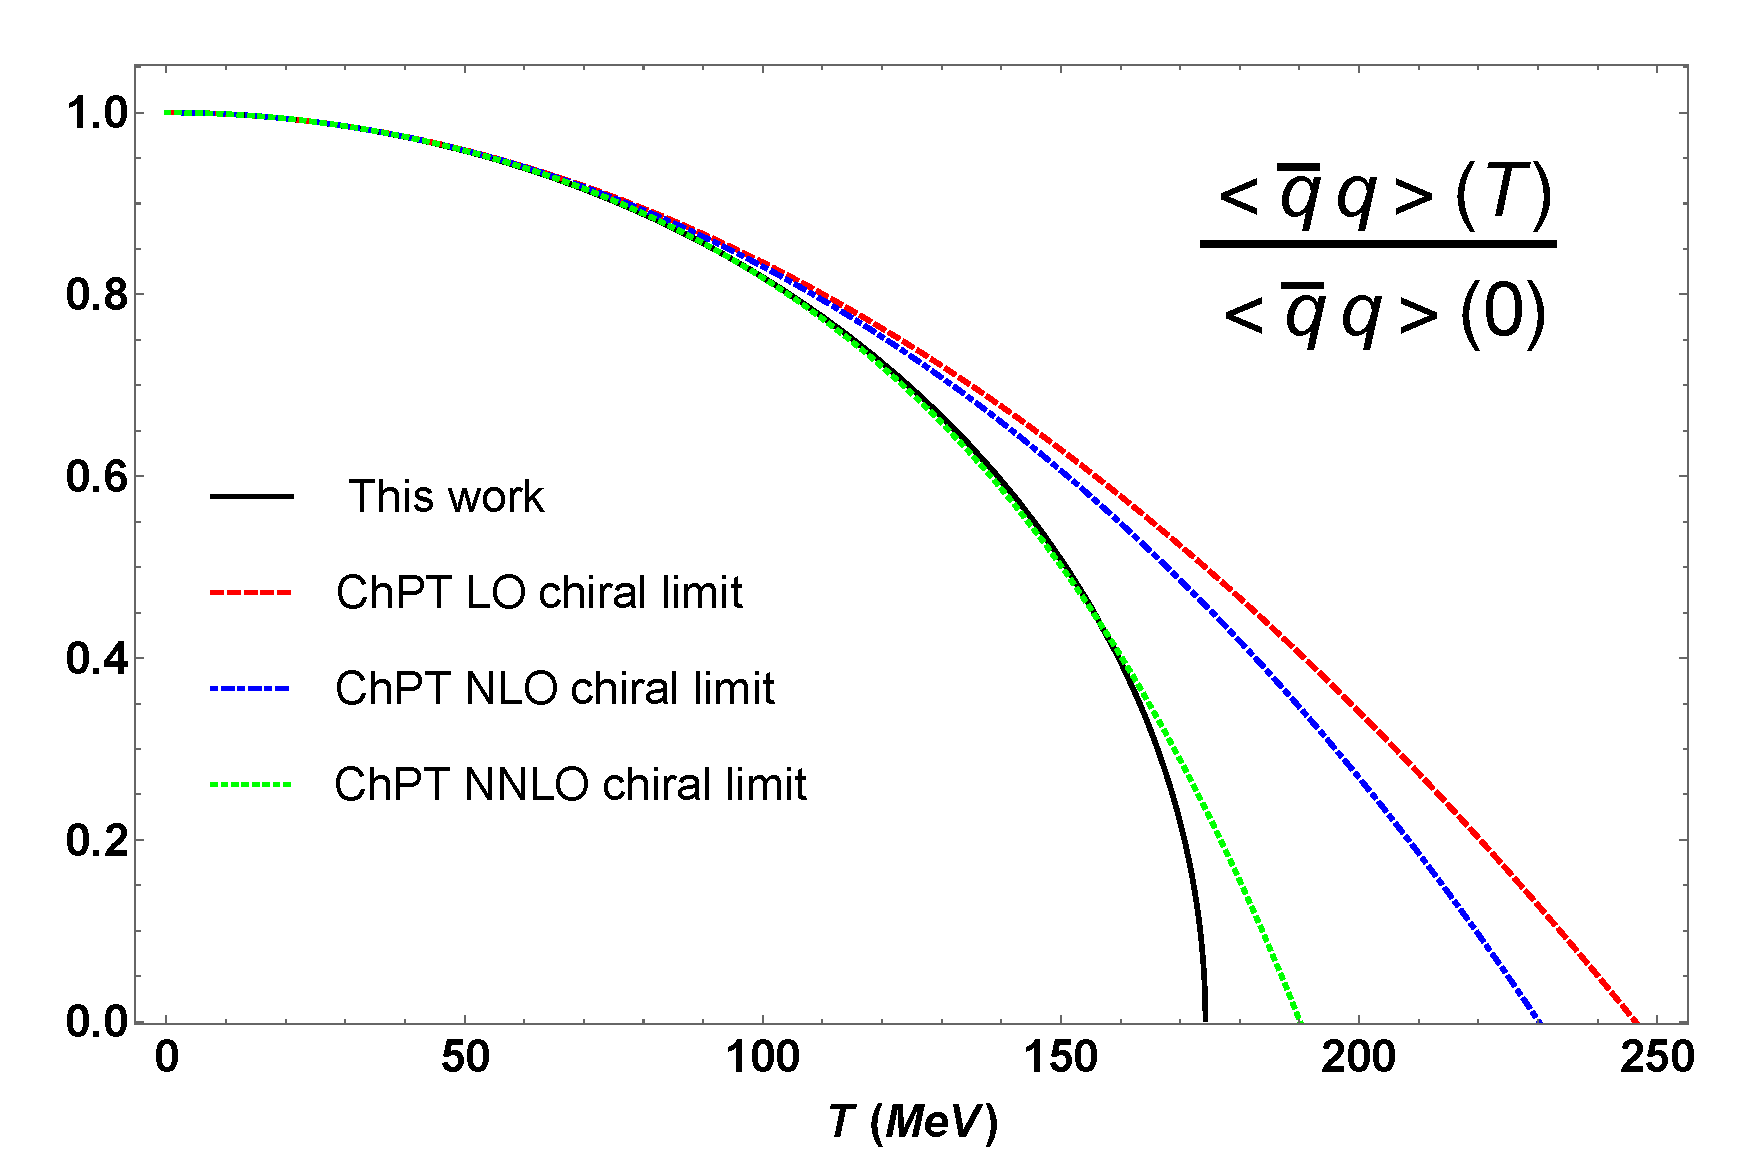
\includegraphics[width=.54\linewidth]{plotcond2.pdf} 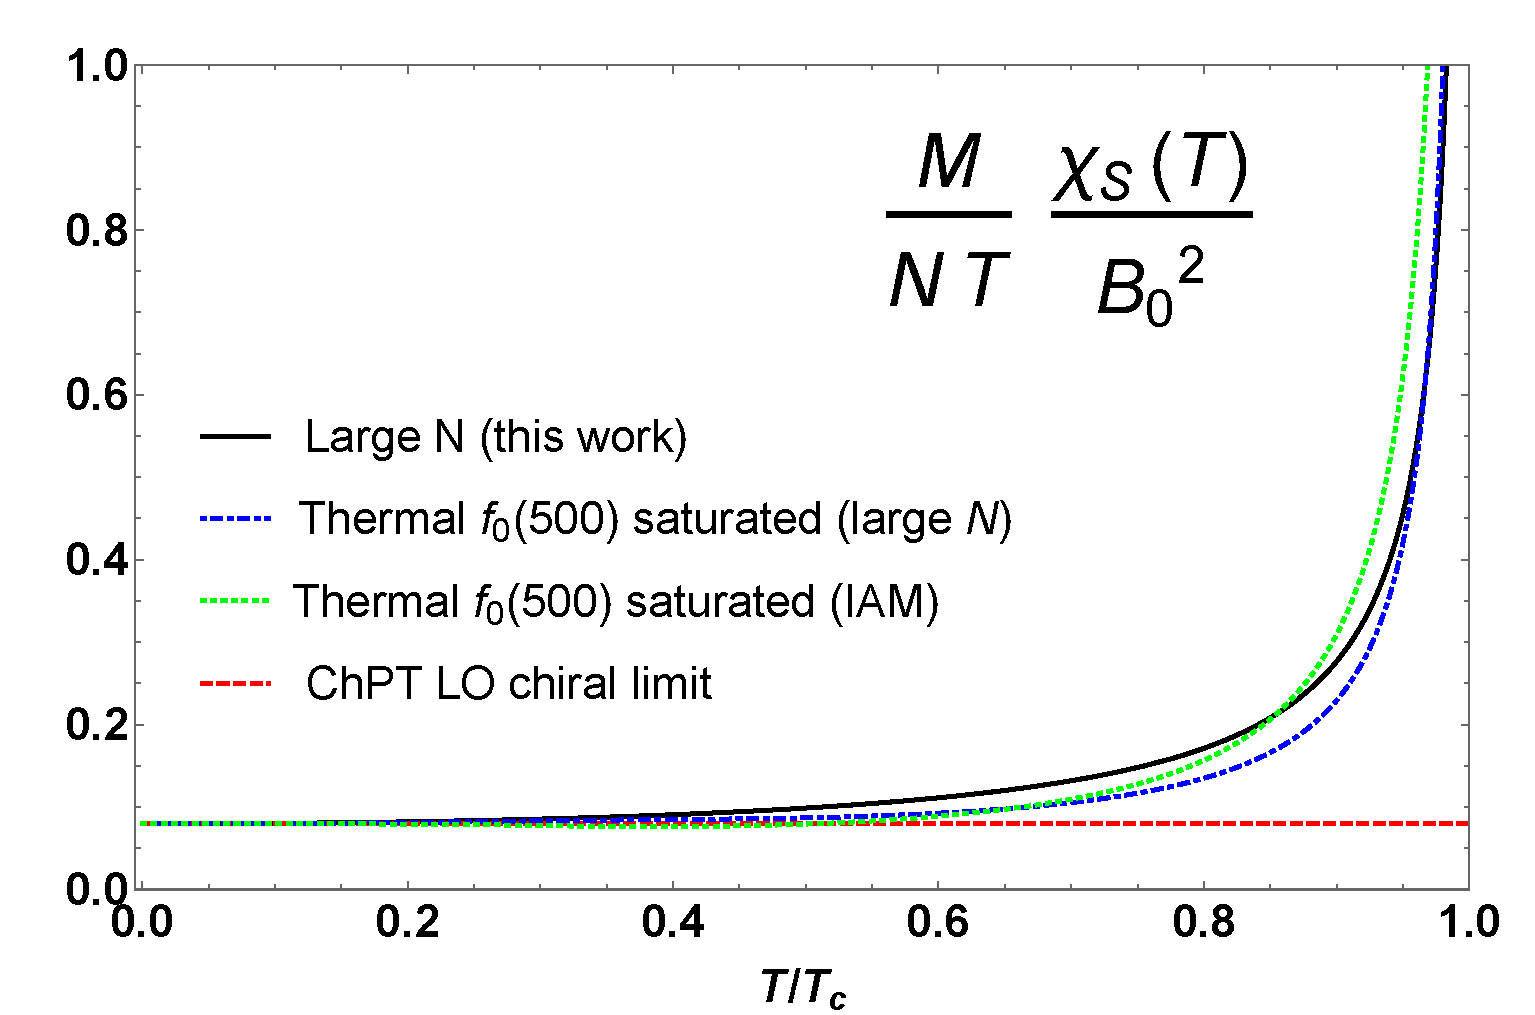
\includegraphics[width=.56\linewidth]{plotsus.pdf}}
\end{center}
\label{fig:partfun}
\end{figure}

\vspace{-0.5cm}

\blindtext

\section{Conclusions} 

\blindtext

\bibliographystyle {plain} 
\begin{thebibliography}{10}

\bibitem{Aoki:2009sc}
  Y.~Aoki, S.~Borsanyi, S.~Durr, Z.~Fodor, S.~D.~Katz, S.~Krieg and K.~K.~Szabo,
  %``The QCD transition temperature: results with physical masses in the
  %continuum limit II,''
  JHEP {\bf 0906}, 088 (2009).
  %[arXiv:0903.4155 [hep-lat]].
	
%\cite{Dobado:1994fd}
\bibitem{Dobado:1994fd} 
  A.~Dobado and J.~Morales,
  %``Pion mass effects in the large N limit of chi(PT),''
  Phys.\ Rev.\ D {\bf 52}, 2878 (1995).
%  [hep-ph/9407321].
  %%CITATION = HEP-PH/9407321;%%
	
	
\bibitem{Gerber:1988tt}
  P.~Gerber and H.~Leutwyler,
  %``Hadrons Below the Chiral Phase Transition,''
  Nucl.\ Phys.\  B {\bf 321}, 387 (1989).
	
	
%\cite{Cortes:2016ecy}
\bibitem{Cortes:2016ecy} 
  S.~Cort\'es, A.~G\'omez Nicola and J.~Morales,
  %``Chiral Symmetry Restoration for the large-$N$ pion gas,''
  Phys.\ Rev.\ D {\bf 94}, no. 11, 116008 (2016).
  %doi:10.1103/PhysRevD.94.116008
  %[arXiv:1609.07751 [hep-ph]].
  %%CITATION = doi:10.1103/PhysRevD.94.116008;%%
  %2 citations counted in INSPIRE as of 25 Aug 2017
	

%\cite{Cortes:2015emo}
\bibitem{Cortes:2015emo} 
  S.~Cort\'es, A.~G\'omez Nicola and J.~Morales,
  %``Large-$N$ pion scattering at finite temperature: the $f_0(500)$ and chiral restoration,''
  Phys.\ Rev.\ D {\bf 93}, no. 3, 036001 (2016).
  %doi:10.1103/PhysRevD.93.036001
  %[arXiv:1511.00031 [hep-ph]].
  %%CITATION = doi:10.1103/PhysRevD.93.036001;%%
  %4 citations counted in INSPIRE as of 25 Aug 2017
	
\end{thebibliography} 
 \end{multicols} 
 \end{document}